\documentclass{article}
\usepackage[utf8]{inputenc}
\usepackage[top=0.75in, bottom=0.75in, left=0.65in, right=0.65in]{geometry}
\usepackage{graphicx}
\usepackage{amsmath}
\usepackage{amsmath}
\usepackage{amssymb}
\usepackage{listings}
\usepackage[T1]{fontenc}
\usepackage[lighttt]{lmodern}
\usepackage{filecontents}       % For the example data
\usepackage{pgfplotstable}
\usepackage{array}      % For aligining at decimal point
\usepackage{siunitx}
\usepackage{booktabs}

\usepackage{xcolor}
 
\definecolor{codegreen}{rgb}{0,0.6,0}
\definecolor{codegray}{rgb}{0.5,0.5,0.5}
\definecolor{codepurple}{rgb}{0.58,0,0.82}
\definecolor{backcolour}{rgb}{0.95,0.95,0.92}
 
\lstdefinestyle{mystyle}{
    backgroundcolor=\color{white},   
    commentstyle=\color{codegreen},
    keywordstyle=\color{magenta},
    numberstyle=\tiny\color{codegray},
    stringstyle=\color{codepurple},
    basicstyle=\ttfamily\footnotesize,
    breakatwhitespace=false,         
    breaklines=true,                 
    captionpos=b,                    
    keepspaces=true,                 
    numbers=left,                    
    numbersep=5pt,                  
    showspaces=false,                
    showstringspaces=false,
    showtabs=false,                  
    tabsize=2
}

\lstset{style=mystyle}
\usepackage{graphicx}
\graphicspath{{figure/}}


\newcommand*\lstinputpath[1]{\lstset{inputpath=#1}}
\lstinputpath{codes}
\title{Home Work 02: EAS 520}
\author{Sayem Khan}
\date{Tuesday, October 22, 2019}

\begin{document}

\maketitle
\subsection*{Task 1}
\subsubsection*{Problem a} 
Write a C, C++ or Fortran program that computes this Monte Carlo approximation to $\pi$ for $N = 10^k$
\subsubsection*{Solution}
The problem is given below:
\subsubsection*{Solution}
\lstinputlisting[
  language   = C++,
  basicstyle = \ttfamily,
  frame      = single,
  caption    = {Code for Monte Carlo approximation to $\pi$},
]{monteCarlopi.cpp}


\subsubsection*{Problem b } 
Plot N vs absolute error $|\pi - \pi_N|$ on a log-log plot.  
\subsubsection*{Solution}
\begin{figure}[h!]
  \centering
    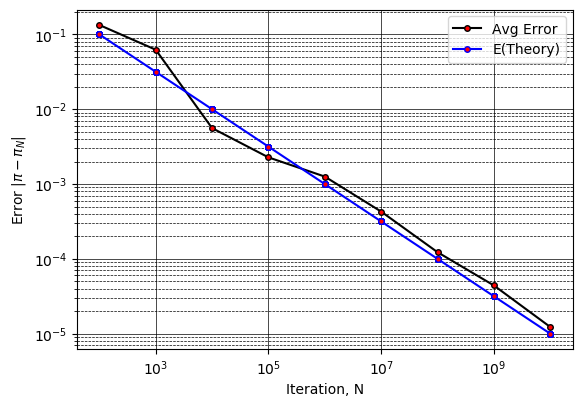
\includegraphics[width=0.85\textwidth]{avg_Err_vs_Iteration.png}
    \caption{Numerical Integration Err vs Iteration: Problem a, Task 1} 
    \label{t1a}
\end{figure}
Here, The program run for $50$ times for a each data and average error is taken. Also, the theoretical relation between error and iteration of MC method, i.e., $E\propto T^{-1/2}$ is also plotted. Comparing to the theoretical limit and calculated limit, it can be error is decreasing at the correct rate.
\lstinputlisting[
  language = bash,
  basicstyle = \ttfamily,
  frame      = single,
  caption    = {Bash script \textbf{avgData.sh} for Problem b, Task 1 },
]{avgData.sh}

\subsubsection*{Problem c } 
Error vs runtime calculation.
\subsubsection*{Solution}
\begin{figure}[h!]
  \centering
    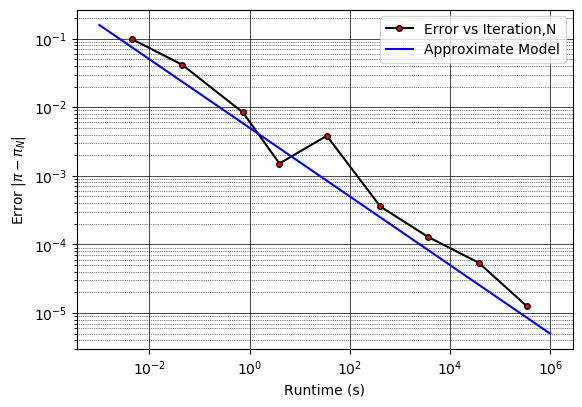
\includegraphics[width=0.85\textwidth]{Error_vs_wall_time_curve.png}
    \caption{Numerical Integration Err vs Iteration: Problem c, Task 1} 
    \label{t1c}
\end{figure}
For the data suing linear regression, it is found that, for accuracy level $E = 10^{-16}$, the program will take $10^{27}$ second (only!) and for $E = 10^{-70030}$ it will take (only!) $10^{140026}$ seconds! Using theoretical calculation and trial-error, best model is $E \propto T^{-1/2}$.  \\
\\
For the calculating the required time, C++ library is used rather than Linux \textbf{time} command. The code is given below:
\lstinputlisting[
  language = C++,
  basicstyle = \ttfamily,
  frame      = single,
  caption    = {Code for Problem c, Task 1 (Only the focused part) },
]{time_short.cpp}
This program is run 10 times for each $N= 10^k$ and average value for runtime and error is taken.
The driver program for this operation is given below:
\lstinputlisting[
  language = bash,
  basicstyle = \ttfamily,
  frame      = single,
  caption    = {Bash script \textbf{time.sh} for Problem c, Task 1 },
]{time.sh}


\subsection*{Task 2}
\subsubsection*{Problem a}
Plotting the likelihood function for model 1
\begin{equation}
    L(x_1,x_2;M_1) = e^{-(1-x_1)^2 - 100(x_2-x_1^2)^2}
    \label{m1}
\end{equation}
\subsubsection*{Solve a} 
We can rewrite the equation \ref{m1} as,
\begin{equation}
    ln(L(x_1,x_2;M_1)) = -(1-x_1)^2 - 100(x_2-x_1^2)^2
    \label{m2}
\end{equation}
Contour plot for equation \ref{m2} is given below:
\begin{figure}[h!]
  \centering
    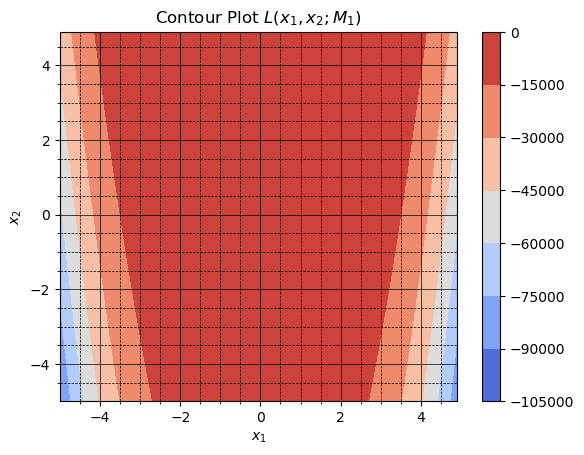
\includegraphics[width=0.75\textwidth]{Contour_plot.png}
    \caption{Contour plot for \ref{m1}} 
    \label{contour}
\end{figure}
The model’s degeneracy will show up as lines
in the x$_1-x_2$ plane where the value of $ L(x_1,x_2;M_1) = e^{-(1-x_1)^2 - 100(x_2-x_1^2)^2}$ does not change.
\begin{figure}[h!]
  \centering
    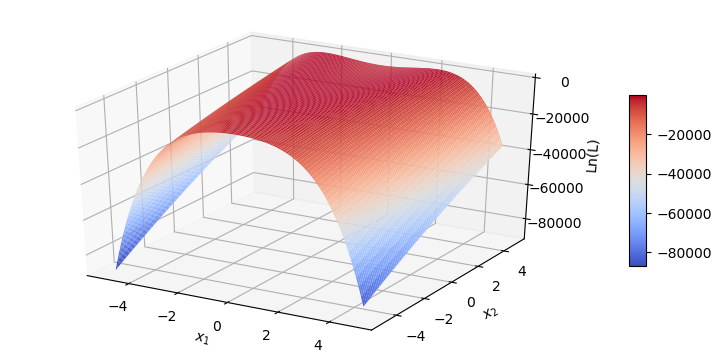
\includegraphics[width=0.9\textwidth]{Contour_plot_3d.png}
    \caption{3D plot for \ref{m1}} 
    \label{contour}
\end{figure}

\subsubsection*{Problem b \& c}
Using Monte Carlo compute, 
$$Z_1 = \int_{-5}^{5}\int_{-5}^{5} L(x_1, x_2; M_1)$$
\subsubsection*{Solve b \& c}
C++ code is give below: 
\lstinputlisting[
  language = C++,
  basicstyle = \ttfamily,
  frame      = single,
  caption    = {Code for Problem b \& c, Task 2 },
]{likelihood_fqn.cpp}
The driver program for this operation is given below:
\lstinputlisting[
  language = bash,
  basicstyle = \ttfamily,
  frame      = single,
  caption    = {Bash script \textbf{time.sh} for Problem a \& c, Task 2},
]{likelihood.sh}
The values of $Z_1$ and $ln(Z_1)$ is given below: 
\begin{center}

\begin{filecontents}{likelihood.csv}
N,Z1,ln(Z1)
100,0.517913,-0.657948
1000,0.317282,-1.14796
10000,0.270797,-1.30639
100000,0.29388,-1.22458
1000000,0.297553,-1.21216
10000000,0.300579,-1.20205
100000000,0.301705,-1.19831
1000000000,0.301509,-1.19896
10000000000,0.301561,-1.19878
\end{filecontents}
% \pgfplotstableread[col sep=comma]{likelihood.csv}{\table}
% \pgfplotstabletypeset[
%     dec sep align,      % Align at decimal point
%     fixed zerofill,     % Fill numbers with zeros
%     precision=4,        % Set number of decimals
%     display columns/0/.style={precision=1}, % Change for first column (column 0)
%     ] {\table}
\pgfplotstableread[col sep=comma]{likelihood.csv}{\table}

\pgfplotstabletypeset[
    dec sep align=S,    % Use the siunitx `S` column type for aligning at decimal point
    %fixed zerofill,     % Fill numbers with zeros
    precision=15,        % Set number of decimals
    display columns/0/.style={
        %precision=1,    % Change for first column (column index 0)
        column name=$N$
    },
    display columns/1/.style={column name=$Z_{1}$},
    display columns/2/.style={column name=$ln{Z_1}$},
    every head row/.style={before row=\toprule, after row=\midrule},
    every last row/.style={after row=\bottomrule},
    ] {\table}
\end{center}
From the above table, for 2 digit precision the N value should be around $10^7$.

\subsubsection*{Problem d}
Compare the runtime between stampede2 and my Laptop.
\subsubsection*{Solve d}
Runtime for $N = 10^9$ of the code:
\begin{enumerate}
    \item My Laptop: $70.42s$
    \item stampede2: $562.6s$
\end{enumerate}
The stampede2 (Model name: Intel(R) Xeon(R) Gold 6132 CPU @ 2.60GHz, CPU(s) = 28
) takes 7.9 times time than my Laptop (Intel(R) Core(TM) i5-6200U CPU @ 2.30GHz
, CPU(s) = 4). The stampede2 is faster than my Laptop, but takes more time!

\subsubsection*{Problem e}
\subsubsection*{Solve e}
For 40 trials my Laptop will take $\frac{(70.42\times 40)}{4} = 704s $ and stampede2 will take
$\frac{(562.6\times 40)}{28} = 803.71s $
\subsubsection*{Problem f}
\subsubsection*{Solve f}
For the 1st likelihood fqn,
\begin{equation*}
    \begin{split}
        Z_1 & = \int_{-5}^{5}\int_{-5}^{5}L(x_1,x_2;M_1)dx_1dx_2 \\
        & = 3:013496893\times 10^{-1};
    \end{split}
\end{equation*}
Here,
\begin{equation*}
    L(x_1,x_2;M_1) = e^{-(1-x_1)^2 - 100(x_2-x_1^2)^2}
    \label{m1}
\end{equation*}

For the 2nd likelihood fqn,
\begin{equation*}
\begin{split}
    Z_1 & = \int_{-5}^{5}\int_{-5}^{5}L(x_1,x_2;M_2)dx_1 dx_2 
    \\
    & = 100
  \end{split}
\end{equation*}
\begin{equation*}
    L(x_1,x_2;M_2) = 1
    \label{m1}
\end{equation*}
Since, $Z_2 > Z_1$, so, $Z_2$ or model 2 fits data better.

\end{document}
